% Asset ID: AS1ExponentialsAndLogarithmsTikZ-002
% Asset type: TikZ diagram
% Suggested file path: tikz/AS1ExponentialsAndLogarithmsTikZ-002.tex
% Unit code: AS1
% Topic code: AS1-EXPLOG
% Topic name: Exponentials and logarithms
% Related lesson section: Core Theory 10 and 11
% Source: Chapter 14 PDF and transcript; CCEA AS1-EXPLOG logarithm and natural logarithm boundary
% Purpose: Show the graph of y = ln x, including domain x > 0, root (1,0), and vertical asymptote x = 0.
\documentclass[tikz,border=8pt]{standalone}
\usepackage{amsmath}
\usepackage{pgfplots}
\pgfplotsset{compat=1.18}
\begin{document}
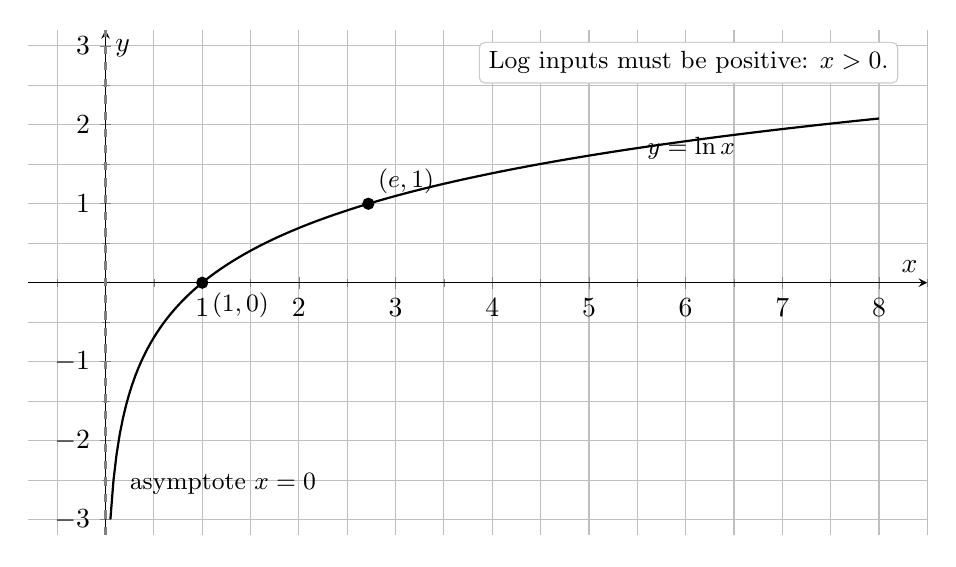
\begin{tikzpicture}
\begin{axis}[width=13cm,height=8cm,axis lines=middle,xmin=-0.8,xmax=8.5,ymin=-3.2,ymax=3.2,xlabel={$x$},ylabel={$y$},grid=both,minor tick num=1,samples=250,domain=0.05:8]
\addplot[dashed,thick,gray] coordinates {(0,-3.2) (0,3.2)};
\addplot[thick]{ln(x)};
\addplot[only marks,mark=*,mark size=2pt] coordinates {(1,0) (2.71828,1)};
\node[anchor=north west,font=\small] at (axis cs:1,0) {$(1,0)$};
\node[anchor=south west,font=\small] at (axis cs:2.71828,1) {$(e,1)$};
\node[anchor=west,font=\small] at (axis cs:5.5,1.7) {$y=\ln x$};
\node[anchor=west,font=\small] at (axis cs:0.15,-2.55) {asymptote $x=0$};
\node[align=left,anchor=north east,font=\small,fill=white,draw=black!20,rounded corners=2pt] at (axis cs:8.2,3.05) {Log inputs must be positive: $x>0$.};
\end{axis}
\end{tikzpicture}
\end{document}
